%%%%%%%%%%%%%%%%%%%%%%%%%%%%%%%%%%%%%%%%%%%%%%%%%%%%%%%%
%%%%%%%%%%%%%%%%%%%%%%%%%%%%%%%%%%%%%%%%%%%%%%%%%%%%%%%%
%  PREAMBLE : USE AT THE BEGINNING OF EVERY PRESENTATION 
%%%%%%%%%%%%%%%%%%%%%%%%%%%%%%%%%%%%%%%%%%%%%%%%%%%%%%%%
%%%%%%%%%%%%%%%%%%%%%%%%%%%%%%%%%%%%%%%%%%%%%%%%%%%%%%%%
\documentclass[11pt]{beamer}

\usepackage{appendixnumberbeamer}

\usepackage{booktabs}
\usepackage[scale=2]{ccicons}

\usepackage{pgfplots}
\usepgfplotslibrary{dateplot}

\usepackage{fontspec}
\defaultfontfeatures{Ligatures=TeX}
\setsansfont{Roboto}[
    Path = /usr/local/texlive/2017/texmf-dist/fonts/truetype/google/roboto/,
    Extension =.ttf,
    ItalicFont = *-RegularItalic,
    BoldFont = *-Black,
    UprightFont = *-Regular ]

% set beamer fonts
\setbeamerfont{title}{size=\Huge}
% \setbeamerfont{itemize/enumerate body}{size=\large}
% \setbeamerfont{itemize/enumerate subbody}{size=\normalsize}
% \setbeamerfont{itemize/enumerate subsubbody}{size=\small}
\setbeamerfont{frametitle}{size=\Large}
\DeclareMathSizes{14}{14.5}{11}{11}

% Change default title color
\usepackage{xcolor}
\definecolor{myblue}{RGB}{18, 65, 104}  % title color
\definecolor{myhl}{RGB}{21, 126, 186}   % texthighlight color
\definecolor{myblack}{RGB}{43, 40, 40}
\setbeamercolor{titlelike}{parent=structure,fg=myblue}

% Chaneg bullet points
% \setbeamertemplate{itemize items}{\setlength\itemsep{1em}}
\setbeamercolor*{item}{fg=myblue}

% disable navigation
\setbeamertemplate{navigation symbols}{}

% Add progressbar
\setbeamercolor{progress bar progress}{use=progress bar,bg=progress bar.fg}
\defbeamertemplate{footline}{progress bar}{%
    \ifnum\thepage>1\relax
        \dimen0=\paperwidth%
        \multiply\dimen0 by \insertframenumber
        \divide\dimen0 by \inserttotalframenumber
        \edef\progressbarwidth{\the\dimen0}

        \leavevmode%
        \begin{beamercolorbox}[wd=\paperwidth,ht=2.25ex,dp=1ex]{progress bar}
        \begin{beamercolorbox}[wd=\progressbarwidth,ht=2.25ex,dp=1ex]{progress bar progress}
        \end{beamercolorbox}%
    \end{beamercolorbox}%
\fi
}
\setbeamertemplate{footline}[progress bar]
\setbeamercolor{progress bar}{fg=myblue,bg=white!70!black}


% disable "Figure:" in the captions
\setbeamertemplate{caption}{\tiny\insertcaption}
\setbeamertemplate{caption label separator}{}

% set new command for code/highlight
\newcommand{\code}[1]{\texttt{#1}}
\newcommand{\hl}[1]{\textcolor{myhl}{#1}}

% use package for text positioning
\usepackage[absolute,overlay]{textpos}
%%%%%%%%%%%%%%%%%%%%%%%%%%%%%%%%%%%%%%%%%%%%%%%%%%%%%%%%

%----------------
% BEGIN DOCUMENT
%----------------
\graphicspath{{/images/}}

\title{\textbf{Slip on Faults and Stress Inversion}}
\date{Jan 30, 2019}
\author{Prithvi Thakur}

\begin{document}

\maketitle

\linespread{1.3}

\begin{frame}{\textbf{Anderson's Theory of Faulting}}
    \begin{itemize}
        \item Earth's free surface cannot support shear, therefore, one of the principal stresses has to be vertical. \hl{Normal, Reverse, Strike-Slip Faulting}.
    \end{itemize}
    \begin{figure}
        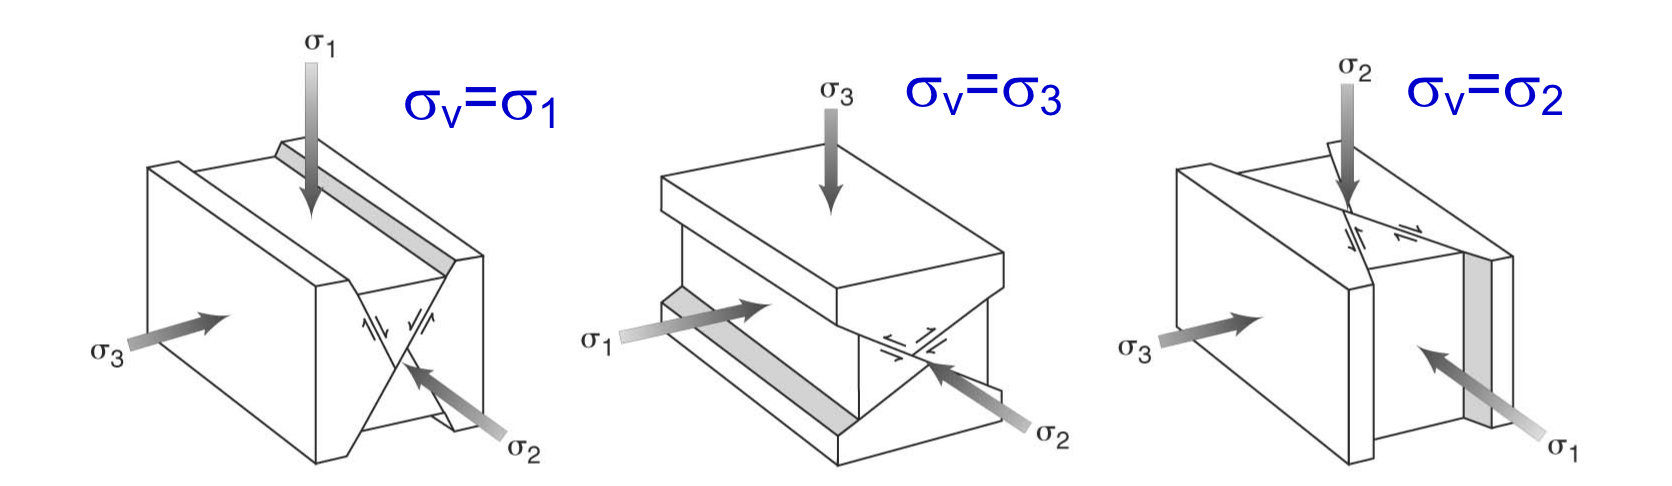
\includegraphics[width=1\linewidth]{images/anderson}
    \end{figure}
\end{frame}

\begin{frame}{\textbf{Anderson's Theory of Faulting}}
    \begin{itemize}
        \item \hl{Limitation:} Only works for intact rocks near the free surface.
        \item \hl{Limitation:} Can't explain low angle normal faults
        \item More realistic faulting style: \hl{oblique-slip faulting}. These occur on pre-existing weakness planes and at a depth, therefore none of the principal stresses are truly vertical.
        \item \hl{Pre-existing weakness:} Reactivated faults, bedding planes, weak layer (shale, salt), foliations, anisotropy in materials, etc.
    \end{itemize}
\end{frame}

\begin{frame}{\textbf{Oblique-slip Faulting}}
    \begin{figure}
        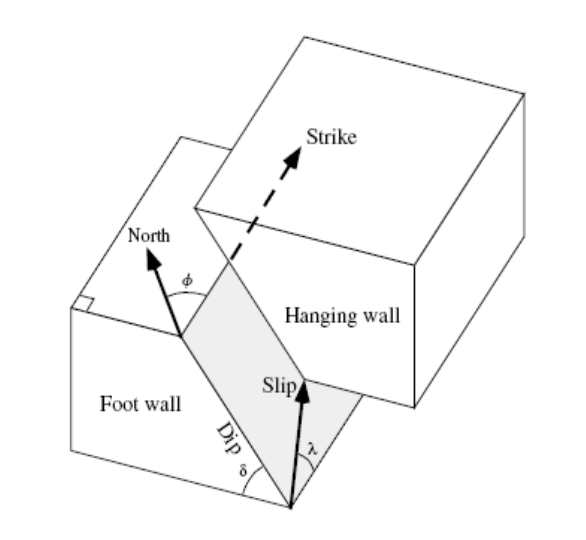
\includegraphics[width=0.6\linewidth]{images/obliquefault}
    \end{figure}
\end{frame}

\begin{frame}{\textbf{Wallace-Bott Hypothesis}}
    Wallace (1951) suggested that \hl{slip on faults occur along the direction and orientation of maximum shear stress}. Bott (1959) derived the equations for the same.
    \\~\\
    Why hypothesis? Due to the following assumptions:
    \begin{itemize}
        \item Faults move during the same tectonic event independently.
        \item No plasticity/ductility during deformation.
    \end{itemize}
\end{frame}

\begin{frame}{\textbf{Fault Geometry}}
    Range of values for: \\
    Strike: $[0,360]$; Dip: $[0,90]$; Rake: $[-90,90]$

    \begin{figure}
        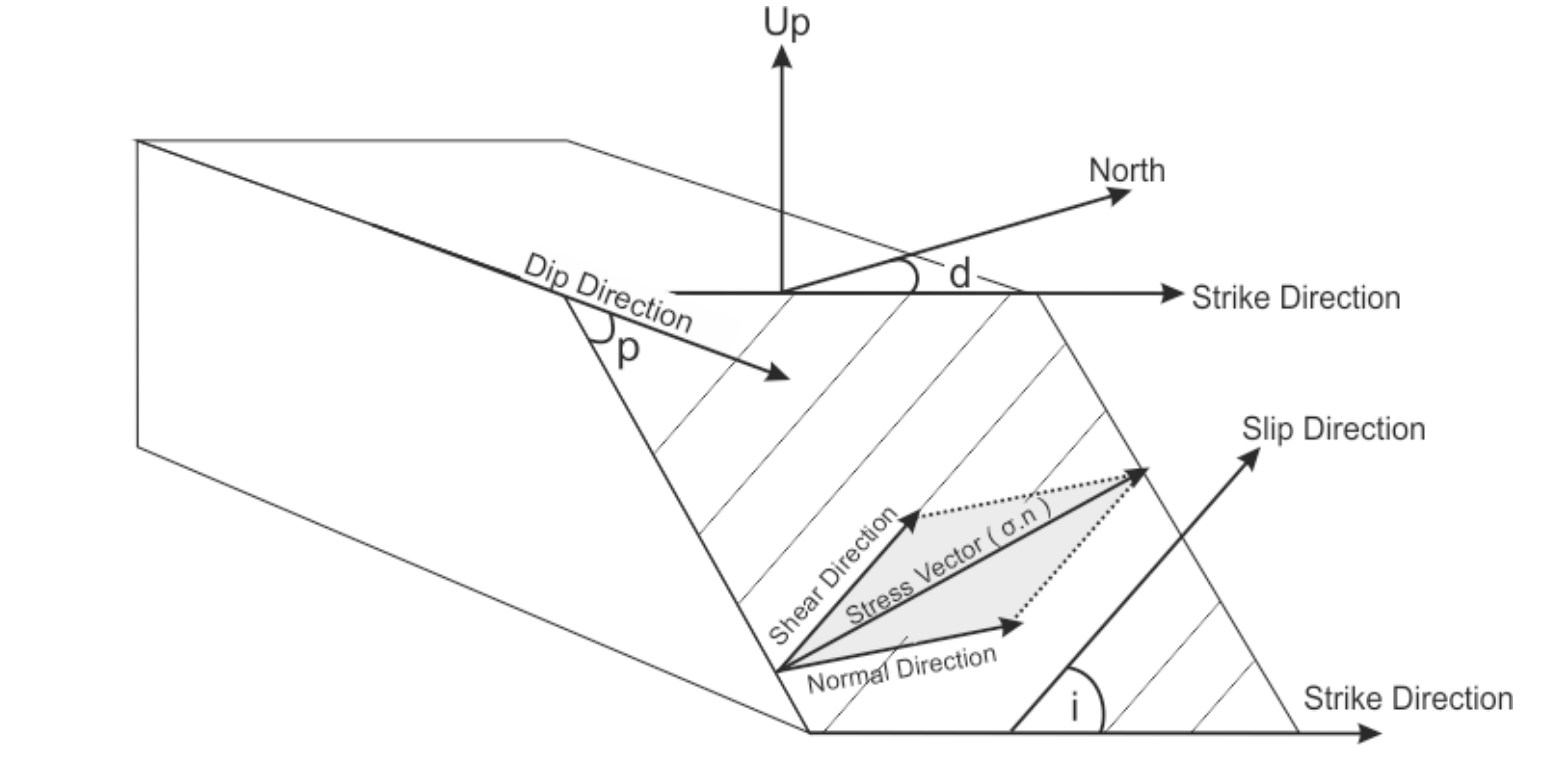
\includegraphics[width=1\linewidth]{images/fault}
    \end{figure}
\end{frame}

\begin{frame}{\textbf{Measuring Fault Slip}}
    We can obtain slip on faults/discontinouities using various methods. All of these can help us constrain stresses.
    \begin{itemize}
        \item<1-> Mesoscale fault outcrops
        \item<2-> Earthquake focal mechanisms
        \item<3-> Borehole breakouts
        \item<4-> Microstructures: Calcite twinning
    \end{itemize}
\end{frame}
\begin{frame}{\textbf{Measuring Fault Slip}}
    We can obtain slip on faults/discontinouities using various methods. All of these can help us constrain stresses.
    \begin{itemize}
        \item Mesoscale fault outcrops
        \item \hl{Earthquake focal mechanisms}
        \item Borehole breakouts
        \item Microstructures: Calcite twinning
    \end{itemize}
\end{frame}

\begin{frame}{\textbf{Earthquake Focal Mechanism}}
    \begin{figure}
        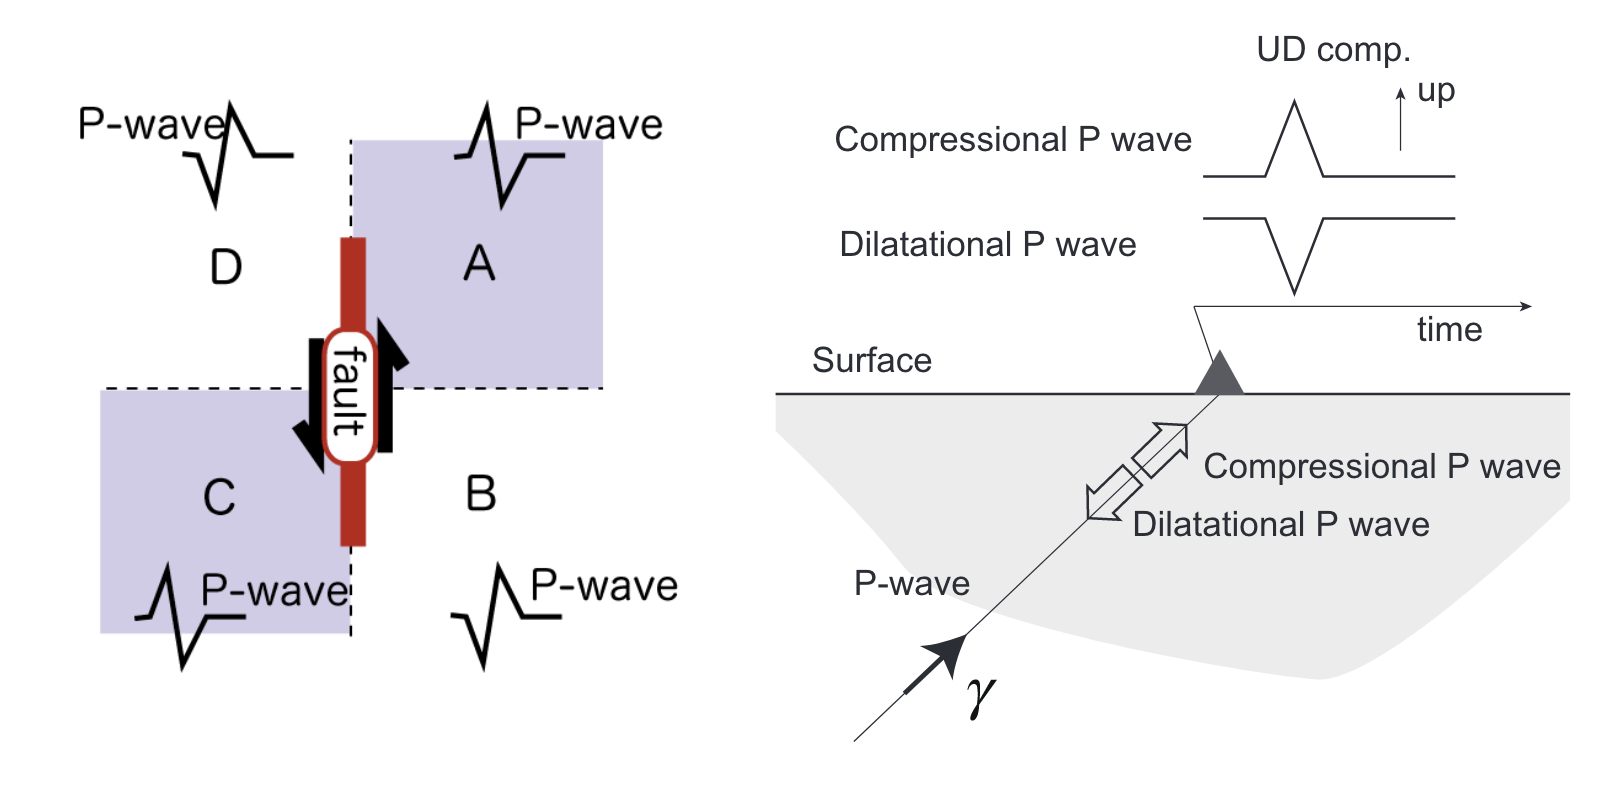
\includegraphics[width=1\linewidth]{images/fm1}
    \end{figure}
\end{frame}
\begin{frame}{\textbf{Earthquake Focal Mechanism}}
    \begin{figure}
        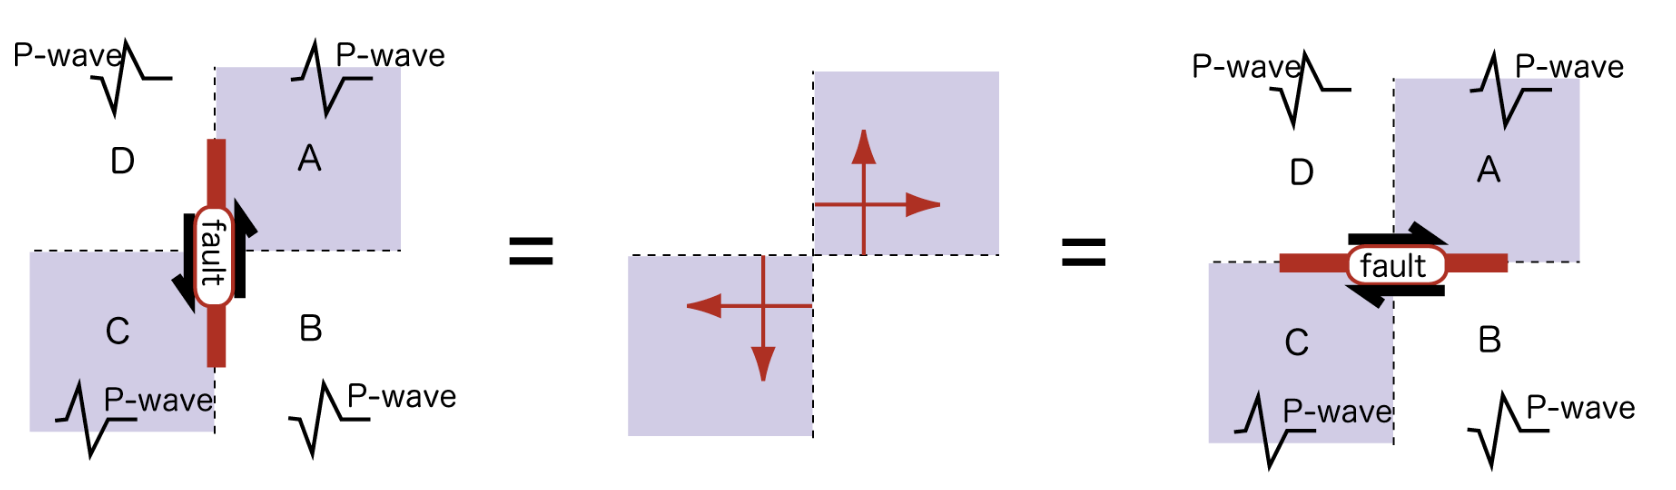
\includegraphics[width=1\linewidth]{images/fm2}
    \end{figure}
\end{frame}
\begin{frame}{\textbf{Stereographic Projection}}
    \begin{figure}
        \includegraphics<1>[width=1\linewidth]{images/stereo2}
        \includegraphics<2>[width=1\linewidth]{images/stereo}
    \end{figure}
\end{frame}
\begin{frame}{\textbf{Earthquake Focal Mechanism}}
        \includegraphics<3>[width=0.5\linewidth]{images/nfm} 
        \includegraphics<1>[width=0.5\linewidth]{images/rfm}
        \includegraphics<2>[width=0.5\linewidth]{images/ssfm}
        \includegraphics<4>[width=0.5\linewidth]{images/osfm}
\end{frame}

\begin{frame}{\textbf{Determining Focal Mechanism}}
    \begin{itemize}
        \item<1-> First motion of P-wave. It can give orientation of fault plane but doesn't give much more information
        \item<2-> Moment Tensor inversion: The representation of source strength and fault orientation. If we assume earth's structure, we can calculate green's function and estimate moment tensor components and location of centroid using waveform inversion.
    \end{itemize}
\end{frame}

\begin{frame}{\textbf{Stress Tensor}}
    \begin{figure}
        \includegraphics<1->[width=0.7\linewidth]{images/stressellipse}
    \end{figure}

    \pause%
    
    Another way of representing stress state just like Mohr's circle. The intersection of any plane passing through the center of this ellipsoid with it would give us the stress vector on that plane.
    \\~\\
    Shape of the stress ellipsoid: stress ratio = $\frac{\sigma_2 - \sigma_3}{\sigma_1 - \sigma_3}$
\end{frame}

\begin{frame}
    \begin{figure}[!htb]
        \centering
        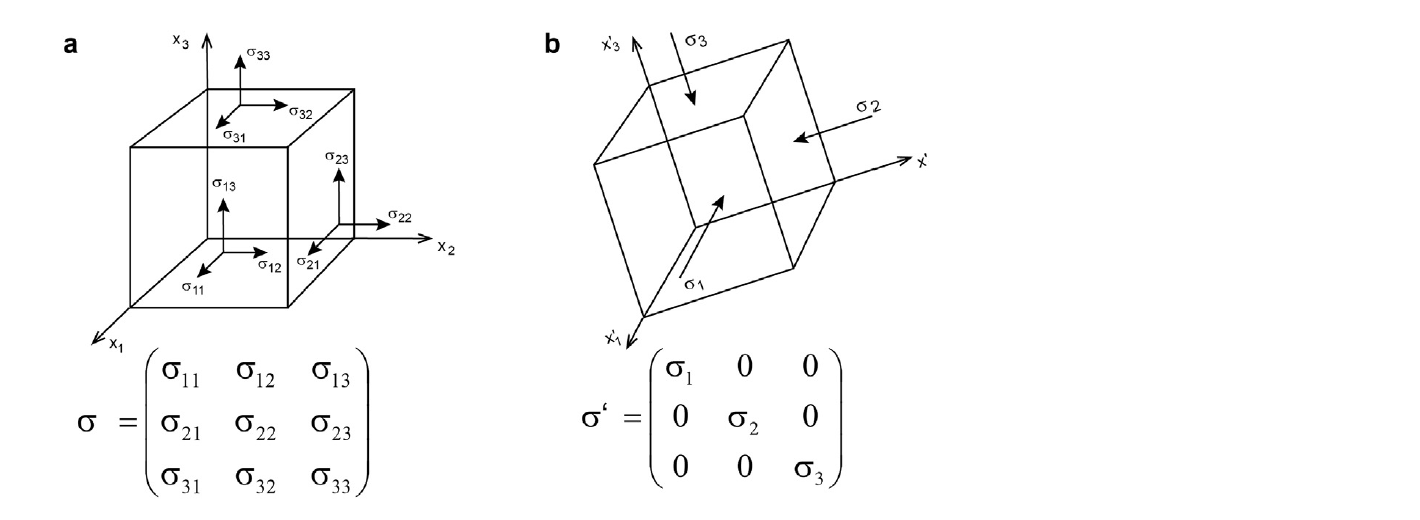
\includegraphics[width=1\linewidth]{images/obliquestress}
    \end{figure}
    \pause%
    \begin{align*}
        \mathbf{\sigma} = \mathbf{R}^T.\mathbf{\sigma'}.\mathbf{R} \\
        \mathbf{\sigma}_0 = (\mathbf{\sigma'} - \mathbf{I}k_1)k_2 \\
        \mathbf{\sigma}_0 = 
        \begin{bmatrix}
            1 & 0 & 0 \\
            0 & \phi & 0 \\
            0 & 0 & 0
        \end{bmatrix}
    \end{align*}
    if $k_1 = 1/(\sigma_1 - \sigma_3)$ and $k_2 = -\sigma_3$ and $\phi = \frac{\sigma_2 - \sigma_3}{\sigma_1 - \sigma_3}$

\end{frame}


\begin{frame}{\textbf{Estimating Stresses}}
    \begin{itemize}
        \item<1->\hl{Forward Problem}: Given a stress tensor, compute the slip on multiple faults with different orientations.
        \item<2->\hl{Inverse Problem}: Given slip on a fault plane and the orientation of fault plane, we can calculate four out of the six components of the principal stress tensor. For the other two components, we need more information like the pore fluid pressure and the depth of burial of the fault.
\end{itemize}
\end{frame}
\begin{frame}{\textbf{Estimating Stresses}}
    \begin{columns}[t]
        \column{.6\textwidth}
            \begin{figure}
                \includegraphics<1->[width=1\linewidth]{images/fault}
            \end{figure}
        \column{.4\textwidth}
            \begin{itemize}
                \item<2-> $\mathbf{\sigma}.\mathbf{n} = \mathbf{T}$
                \item<3-> $(\mathbf{T}.\mathbf{n})\mathbf{n}$ = the normal component
                \item<4-> $\mathbf{T}-$ normal component = shear component
            \end{itemize}
    \end{columns}
    
\end{frame}

\begin{frame}{\textbf{Estimating Stresses}}
    \begin{itemize}
        \item<1-> \hl{Input parameters}: Strike, dip, rake. This implies we know the normal vector the slip vector for each fault plane.
        \item<2-> Compute the theoretical slip direction for each of the given fault plane using arbitrary stress tensor.
        \item<3-> Minimize the misfit between theoretical and observed slip direction.
        \item<4-> Depending on the inversion technique used, update the arbitrary stress tensor till you get the best fit.
    \end{itemize}

\end{frame}

\begin{frame}{\textbf{Practice Session}}
    \large{Stresses along the Sumatra-Andaman subduction zone}
    \begin{figure}
        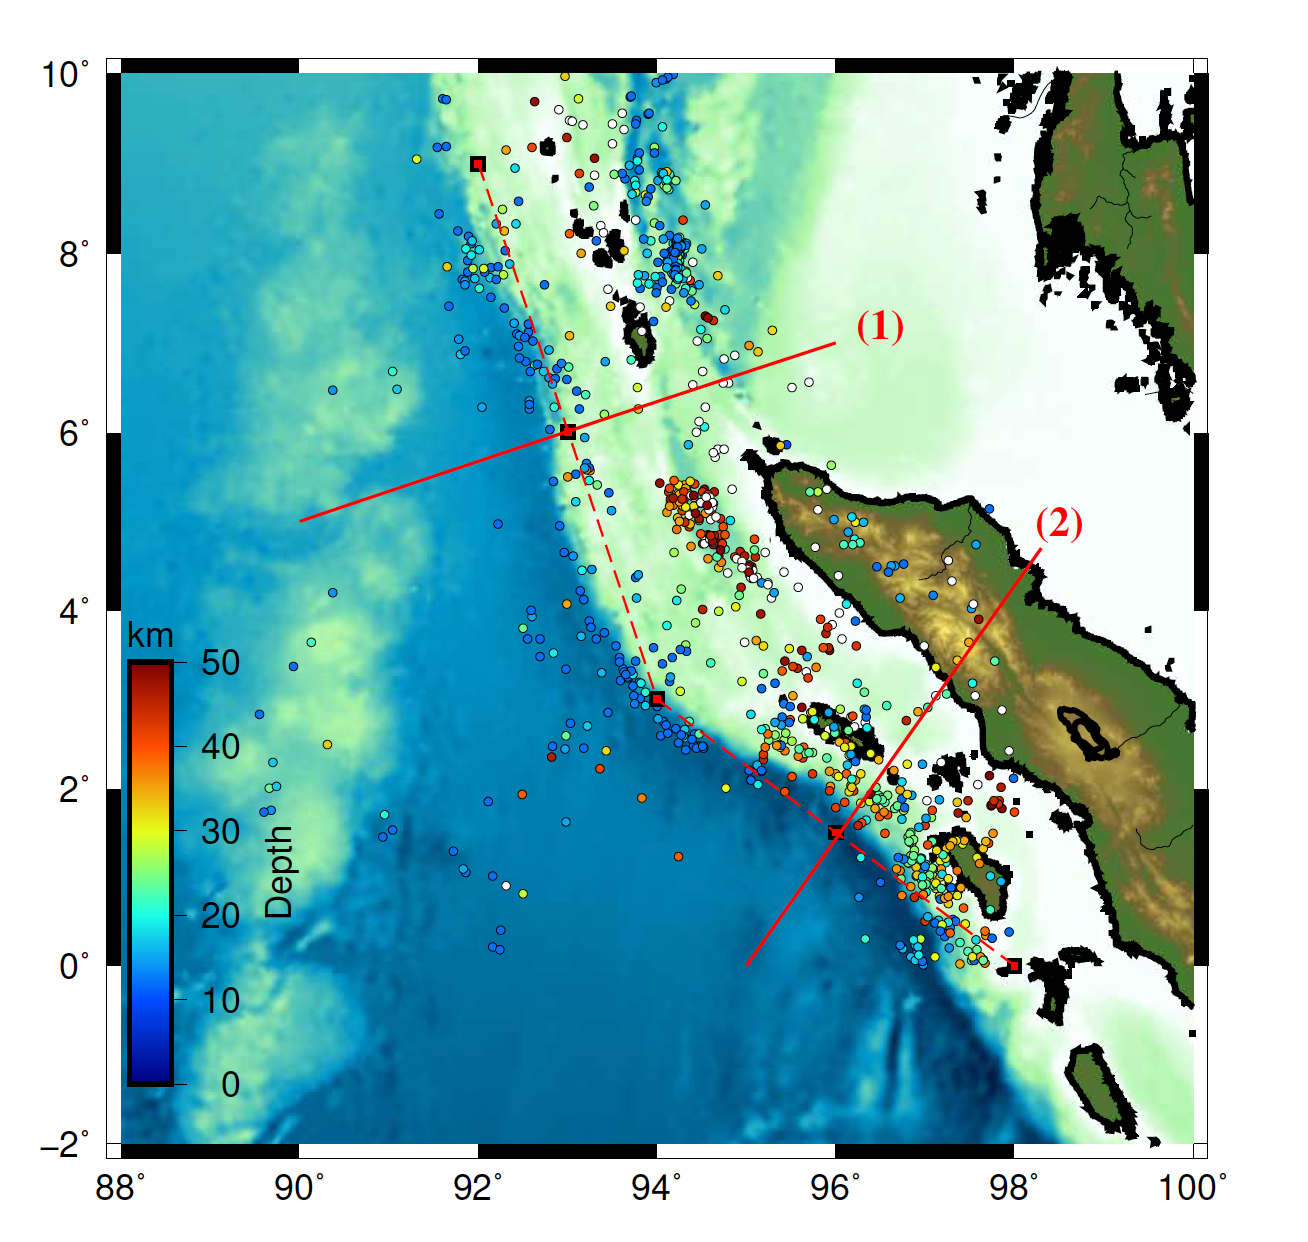
\includegraphics[width=0.6\linewidth]{images/sumatra}
    \end{figure}
\end{frame}

\end{document}
